%themes:    * default * Boadilla * Madrid * Pittsburgh * Rochester         [ works best as \usetheme[height=7mm]{Rochester} ] * Copenhagen * Warsaw * Singapore * Malmoe 
\documentclass[8pt]{beamer}

%setup the theme
\usetheme{Warsaw}
\useoutertheme{infolines} 
%\usetheme[height=7mm]{Rochester} 
\setbeamertemplate{items}[ball]
\setbeamertemplate{blocks}[rounded][shadow=true] 
\setbeamertemplate{navigation symbols}{} 
\usepackage{wasysym}
%algorithm
\usepackage{algorithm}
%for box
\usepackage{fancybox}
%comment a lot of lines
\usepackage{verbatim} 
\usepackage{hyperref}
\usepackage[all]{xy}
%this package will be used for outline
\usepackage{tikz}
\usetikzlibrary{automata,calc,er}
\usetikzlibrary{mindmap,scopes,arrows,arrows.meta,shapes,chains,positioning,fit,backgrounds,decorations,intersections,petri,decorations.pathmorphing}
\usepackage{pgf}
\usepackage{pgfplots}
\pgfplotsset{compat=1.15}
\usetikzlibrary{pgfplots.fillbetween}
\pgfdeclarelayer{ft}
\pgfdeclarelayer{bg}
\pgfsetlayers{bg,main,ft}
\usepackage{graphics}
\usepackage{amssymb}
\usepackage{adjustbox}

%\tikzstyle{block}=[draw opacity=0.7,line width=1.4cm]

\tikzstyle{every picture}+=[remember picture]

\renewcommand{\thefootnote}{}
\newcommand{\specialcell}[2][c]{%
\begin{tabular}[#1]{@{}c@{}}#2\end{tabular}}
\newcommand{\ttrd}{\textcolor{red}}

  \tikzset{%
  highlight/.style={rectangle,rounded corners,fill=red!15,draw,fill opacity=0.5,thick,inner sep=0pt}
  }
  \newcommand{\tikzmark}[2]{\tikz[overlay,remember picture,baseline=(#1.base)] \node (#1) {#2};}
  %
  \newcommand{\Highlight}[1][submatrix]{%
  \tikz[overlay,remember picture]{
  \node[highlight,fit=(left.north west) (right.south east)] (#1) {};}
  }

  %for flowchart
\tikzstyle{decision} = [diamond, draw, fill=blue!20,
    text width=2.5em, text badly centered, node distance=2.5cm, inner sep=0pt]
\tikzstyle{block} = [rectangle, draw, fill=blue!20,
    text width=2em, text centered, node distance=2.5cm, rounded corners, minimum height=2em]
\tikzstyle{line} = [draw, very thick, color=black!50, -latex']
\tikzstyle{cloud} = [draw, ellipse,fill=red!20, node distance=2cm,
    minimum height=2em]
\tikzstyle{round} = [draw, circle, node distance=2cm,
    minimum height=2em]

\usepackage{calc}
\usepackage{fp}


%title page
\title[Reachability Analysis and Revision of Dynamics]{Reachability Analysis and Revision of Dynamics of\\ Biological Regulatory Networks}
\author[X.Chai]{Xinwei Chai}
\institute[LS2N]{
Le Laboratoire des Sciences du Num\'erique de Nantes\\
\'Ecole Centrale de Nantes\\
\texttt{xinwei.chai@ls2n.fr}

\vspace{1cm}
\begin{tabular}{r@{\ \ }l}
\textbf{Rapporteurs :}
& Gilles BERNOT, Professeur des universit\'es,
    Universit\'e C\^ote d'Azur \\
& Pascale LE GALL, Professeur des universit\'es,
    Centrale Sup\'elec \vspace*{1em} \\
\textbf{Examinateurs :}
& B\'eatrice DUVAL, Professeur des universit\'es, Universit\'e d'Angers  \\
& Lo\"ic PAULEV\'E, Charg\'e de recherche,
    LaBRI, UMR CNRS \vspace*{1em} \\
\textbf{Directeur de th\`ese :}
& Olivier ROUX, Professeur des universit\'es,
    \'Ecole Centrale de Nantes \\
\textbf{Co-encadrant de th\`ese :}
& Morgan MAGNIN, Professeur des universit\'es,
    \'Ecole Centrale de Nantes
\end{tabular}

}
\date[May 24, 2019]{May 24, 2019}
\begin{document}

%--- the titlepage frame -------------------------%
\begin{frame}[plain]
  \titlepage
\end{frame}

%\begin{frame}{Positioning of Our Work}
%\begin{adjustbox}{max totalsize={.9\textwidth}{.9\textheight},center}
%    \centering
%    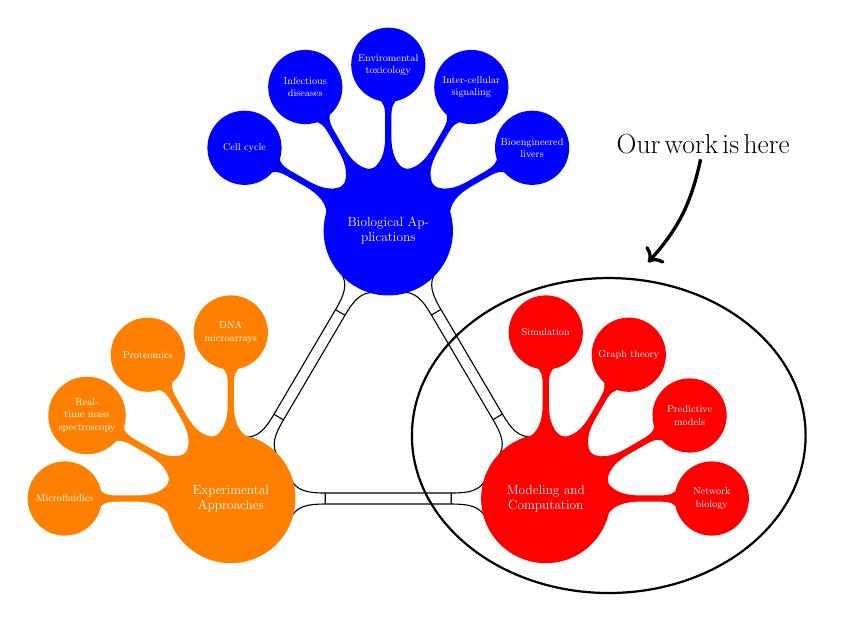
\begin{tikzpicture}[mindmap,
    level 1 concept/.append style={level distance=60,sibling angle=30},
    extra concept/.append style={color=blue!50,text=black}, every node/.style={scale=0.4}]

    \begin{scope}[mindmap, concept color=blue,text=white]
            \onslide<1->{\node [concept] (bioapp) at (2,3.4) {Biological Applications} [counterclockwise from=30] 
            child{node [concept] (bioen) {Bioengineered livers}}
            child{node [concept] (int) {Inter-cellular signaling}}
            child{node [concept] (env) {Enviromental toxicology}}
            child{node [concept] (inf) {Infectious diseases}}
            child{node [concept] (cell) {Cell cycle}};}
    \end{scope}

    \begin{scope}[mindmap, concept color=orange, text=white]
        \onslide<2->{\node [concept] (exp) {Experimental Approaches}[counterclockwise from=90] 
            child{node [concept] (dna) {DNA microarrays}}
            child{node [concept] (prot) {Proteomics}}
            child{node [concept] (rtms) {Real-time mass spectroscopy}}
            child{node [concept] (mic) {Microfluidics}};}
    \end{scope}

    \begin{scope}[mindmap, concept color=red,text=white]
        \onslide<4->{\node [concept] (mod) at (4,0) {Modeling and Computation}[counterclockwise from=0] 
            child{node [concept] (net) {Network biology}}
            child{node [concept] (csm) {Predictive models}}
            child{node [concept] (gra) {Graph theory}}
            child{node [concept] (sim) {Simulation}};}
    \end{scope}

    % Connections of researchers to applied subfields

    \begin{pgfonlayer}{bg}
        \draw<3-> [circle connection bar]
            (exp) edge (bioapp);
        \draw<5-> [circle connection bar]
            (bioapp) edge (mod);
        \draw<6-> [circle connection bar]
            (mod) edge (exp);
    \end{pgfonlayer}
        
    
    \onslide<7>{\node[text width=4cm, align=center] (ellip) at (4.8,0.8) {};
        \draw[thick, draw=black] (ellip) ellipse (2.5 and 2);
      \node (mark) at (6,4.5) [text width=7cm, align=center, inner sep=5pt,minimum size=5pt]  {\Huge{Our work is here}};
      \draw[->,very thick, bend left=15] (mark) edge[->] (5.3,3);}
    
\end{tikzpicture}
%\end{adjustbox}
%\end{frame}
%
%\begin{frame}{Biological Regulatory Networks}
%    \begin{tikzpicture}[-{Latex[length=1.5mm]}]
  \onslide<1->{\node[inner sep=0pt] (cell) {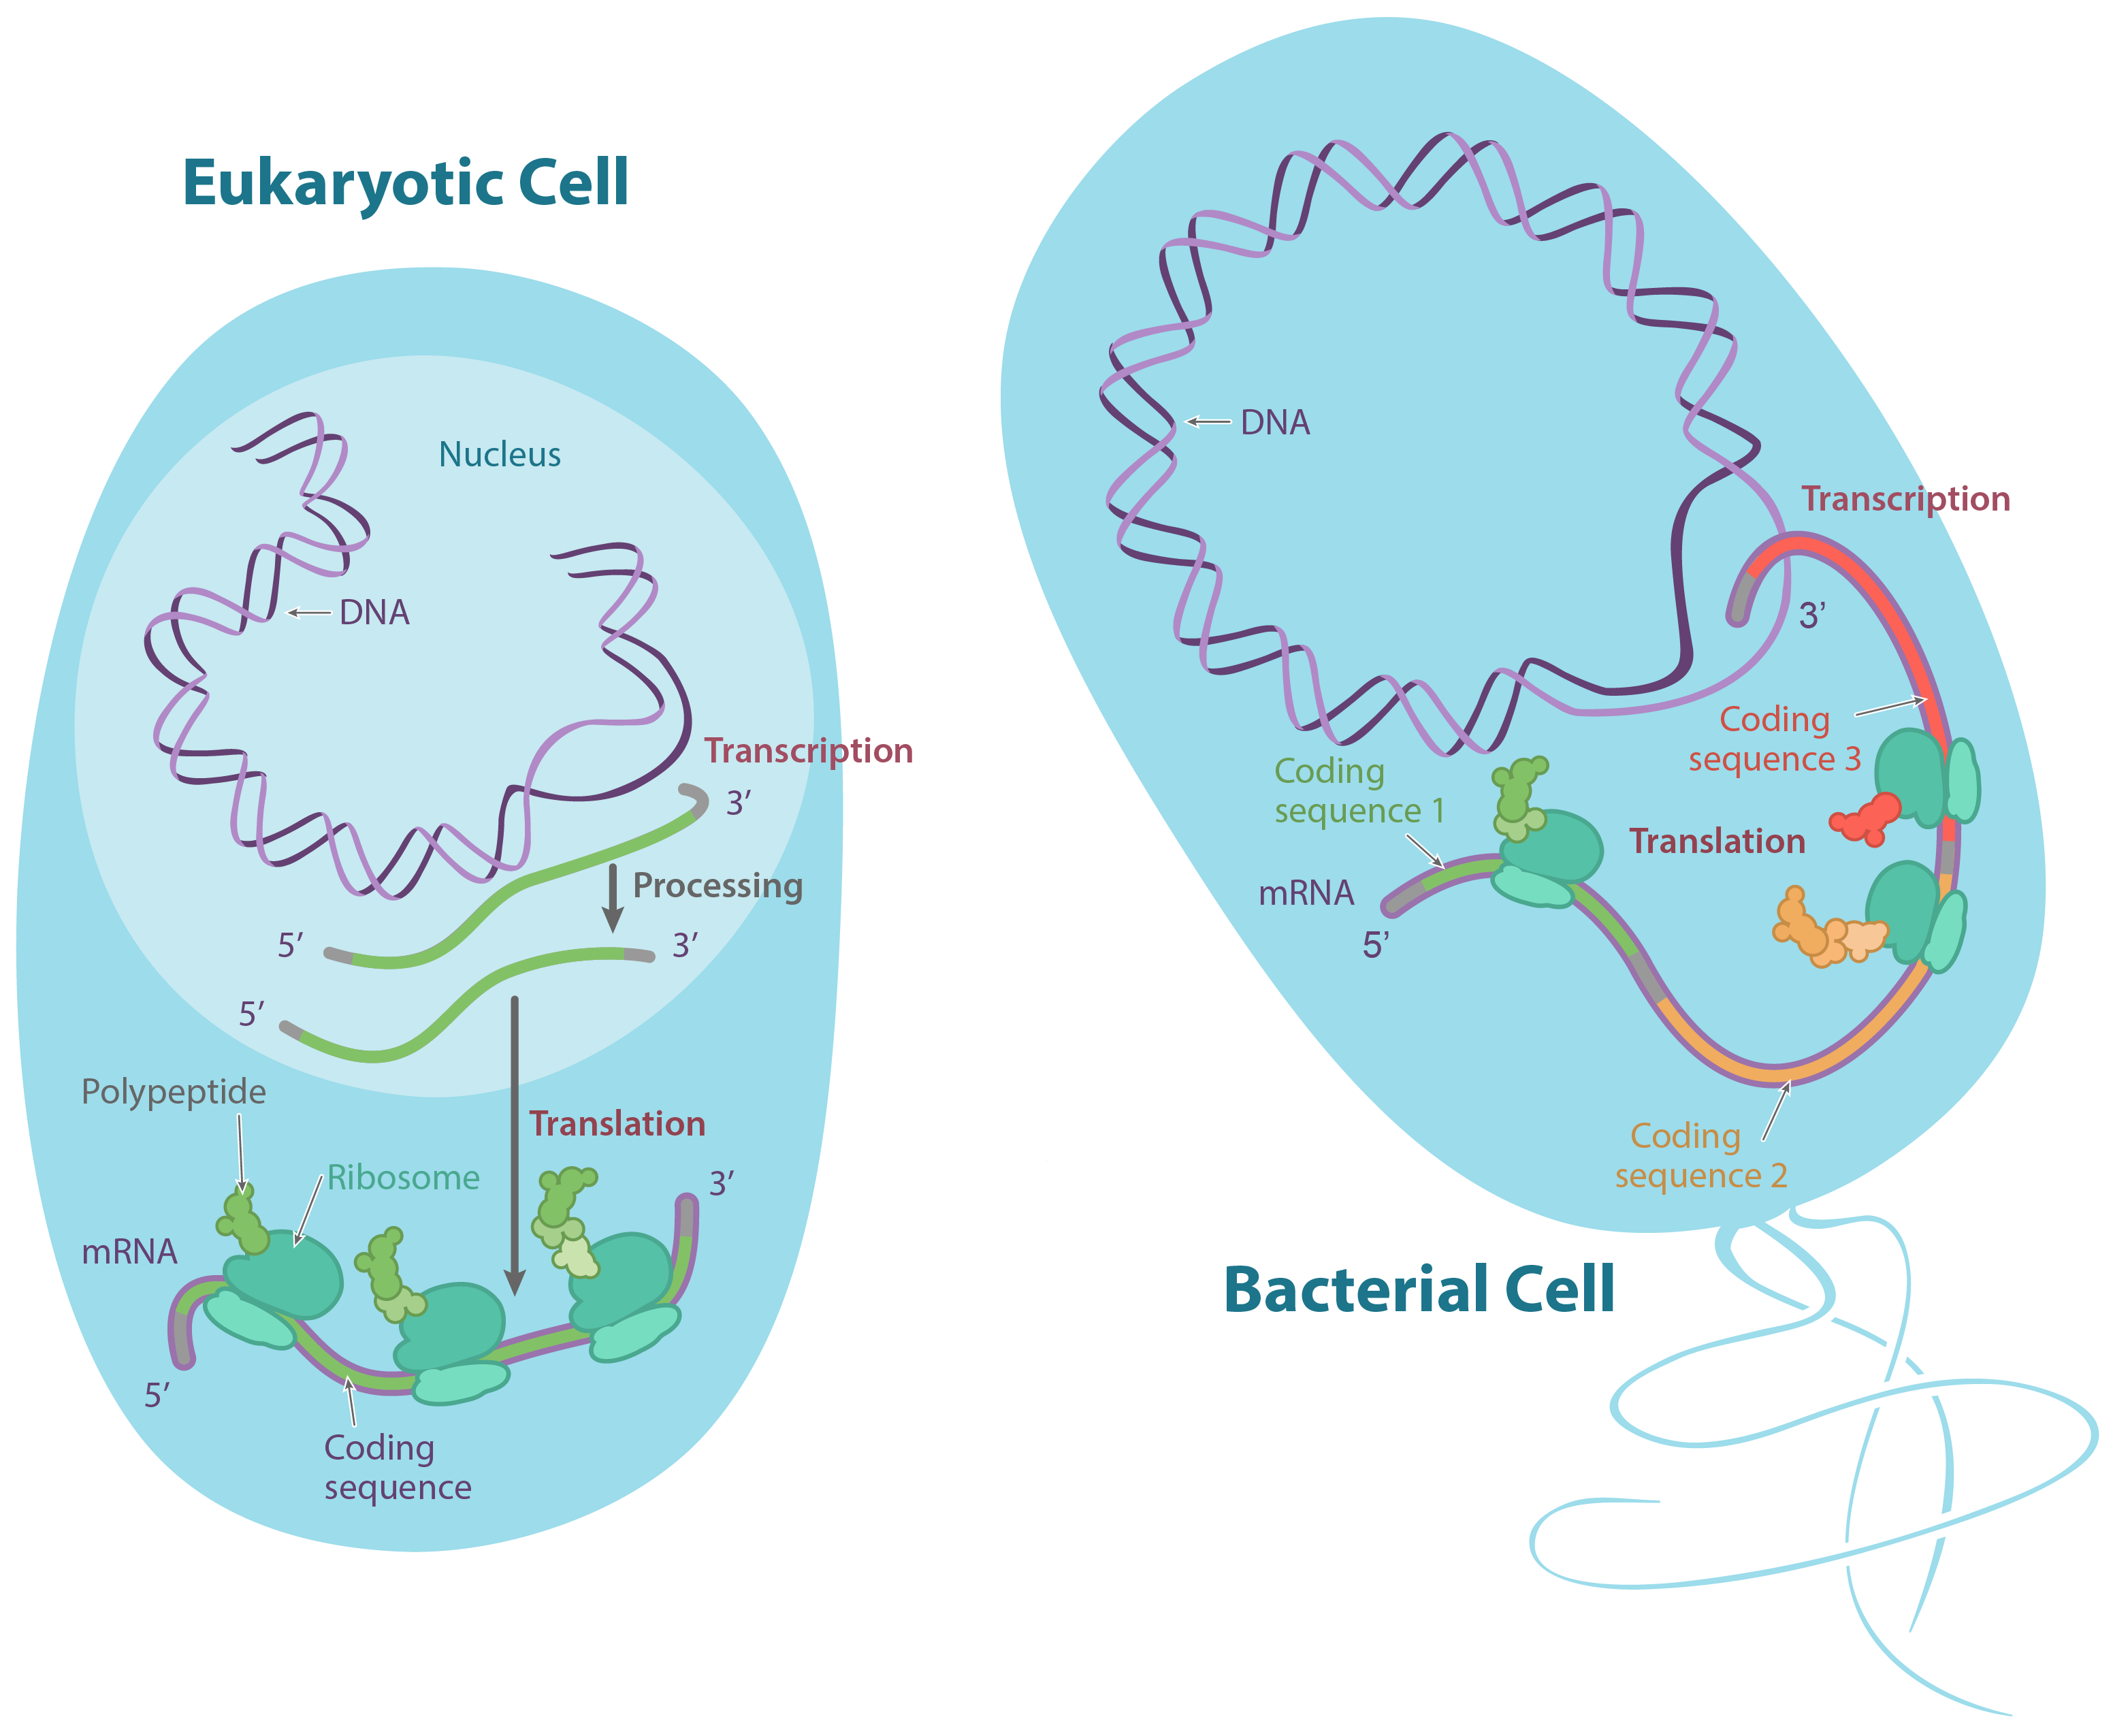
\includegraphics[width=0.45\textwidth]{figures/cell.png}};}
  \onslide<3->{\node[right = of cell] (rnaA)  {\scriptsize RNA of $a$};}
  \onslide<2->{\node[above = of rnaA] (dnaA) {\scriptsize DNA of gene $a$};}
  \onslide<1->{\draw[-latex,thick] (cell) -- (rnaA);}
  \onslide<4->{\node[below = of rnaA] (prA) {\scriptsize Protein of $a$};}
  \onslide<2->{\node[right = of dnaA] (dnaB) {\scriptsize DNA of gene $b$};}
  \onslide<5->{\node[below = of dnaB] (rnaB) {\scriptsize RNA of $b$};}
  \onslide<6->{\node[below = of rnaB] (prB) {\scriptsize Protein of $b$};}
  \onslide<3->{\draw (dnaA) to (rnaA);}
  \onslide<4->{\draw (rnaA) to (prA);}
  \onslide<5->{\draw (dnaB) to (rnaB);}
  \onslide<6->{\draw (rnaB) to (prB);}
  \onslide<10->{\node[draw,dotted,fit=(dnaA) (rnaA) (prA),label=above:$a$] (entityA){};}
  \onslide<11->{\node[draw,dotted,fit=(dnaB) (rnaB) (prB),label=above:$b$] (entityB){};}

  \onslide<7->{\draw[bend right=15, color=blue!50] (prB) to (dnaA);}
  \onslide<8->{\draw[-|,bend left=15,color=red] (prA) to (dnaB);}
  \onslide<9->{\draw[bend right=45, color=blue!50,dashed] (prB) to (dnaB);}
\onslide<13->{
\node (a) [draw,circle,below left = 2cm and 1cm of entityA] {$a$};
\node (b) [draw,circle,right = of a] {$b$};
\draw[-{Latex[length=1.5mm]}, line width=1pt] (a) to[bend left] (b);
\path (b) edge[-|,thick,bend left=30,shorten >=1pt] (a);
\draw[-{Latex[length=1.5mm]}, thick, loop above,dashed] (b) to (b);}
\node[fit=(a)(b)](mid){};
\onslide<12->{\draw[-latex,thick] (prA) -- (mid);}
\onslide<14->{\node [draw=none, right = of b]{How to compute with BRN?};}
\end{tikzpicture}
%\end{frame}
%
%\begin{frame}{Discrete Modeling}
%    \begin{tikzpicture}[scale=0.7]
\scriptsize
    \begin{axis}[samples=100,legend pos=north west,legend style={draw=none}]
        \only<1>{\addplot[mark=none,color=red] function{1/(1+exp(-2*x))};}
        \only<2>{\addplot[mark=none,color=red,domain=-3:0] function{0};}
        \only<2>{\addplot[mark=none,color=red,domain=0:3] function{1};}
        \only<2>{\addplot[fill=white,only marks,mark=*] coordinates{(0,0)(0,1)};}
        \only<1>{\addlegendentry{\normalsize{$\frac{1}{1+e^{-x}}$}}}
        \only<2>{\addlegendentry{$\begin{cases}0,&{\mbox{if }}x<0\\x,&{\mbox{if }}x= 1\end{cases}$}}
    \end{axis}
\end{tikzpicture}
%\end{frame}
%
%%--- the methods part	 -------------------------%
%\section{Motivation}
%\begin{frame}{Problematic of Reachability Problem}
%    \centering
%    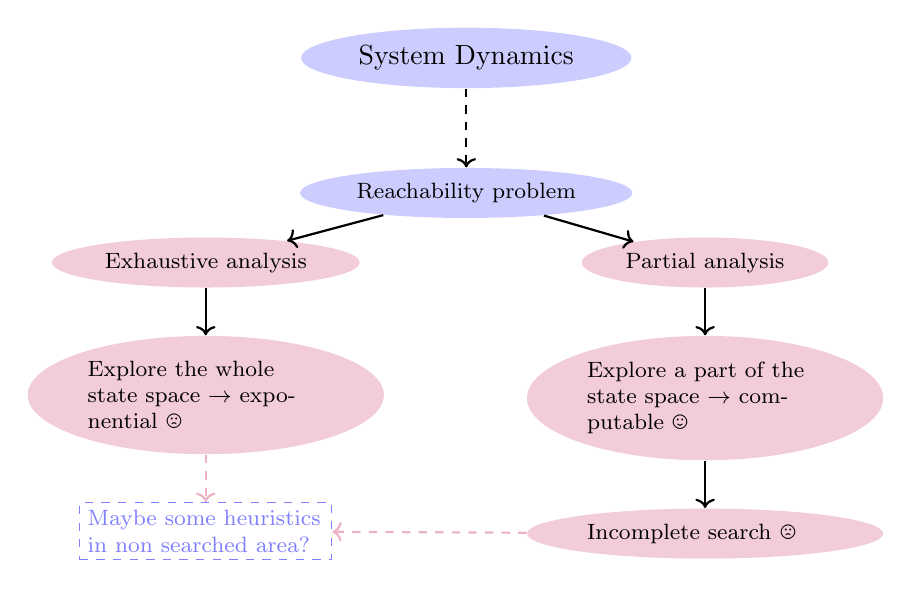
\begin{tikzpicture}
    \onslide<1->{\node[ellipse, fill=blue!20] (dynamics) at (0, 0) {System Dynamics};}
\footnotesize
    \onslide<2->{\node[ellipse, fill=blue!20, below = of dynamics] (reach) {Reachability problem};
    \draw[->,thick,dashed] (dynamics) -- (reach);}
    \onslide<3->{\node[ellipse, fill=purple!20, below left = 0.6cm of reach] (full) {Exhaustive analysis};
    \draw[->,thick] (reach) -- (full);}
    \onslide<5->{\node[ellipse, fill=purple!20, below right = 0.6cm of reach] (part) {Partial analysis};
    \draw[->,thick] (reach) -- (part);}
    \onslide<4->{\node[ellipse, fill=purple!20, below = 0.6cm of full, text width = 3cm] (propfull) {Explore the whole state space $\to$ exponential \frownie{}};
    \draw[->,thick] (full) -- (propfull);}
    \onslide<6->{\node[ellipse, fill=purple!20, below = 0.6cm of part, text width = 3cm] (proppart) {Explore a part of the state space $\to$ computable \smiley{}};
    \draw[->,thick] (part) -- (proppart);}
    \onslide<7->{\node[ellipse, fill=purple!20, below = 0.6cm of proppart, text width = 3cm] (incomp) {Incomplete search \frownie{}};
    \draw[->,thick] (proppart) -- (incomp);}
    \onslide<8->{\node[draw, dashed, color = blue!50, below = 0.6cm of propfull, text width = 3cm] (heu) {Maybe some heuristics in non searched area?};
    \draw[->,dashed, thick, color=purple!30] (incomp) -- (heu);
    \draw[->,dashed, thick, color=purple!30] (propfull) -- (heu);}
    %\draw[thick,blue,rounded corners=1mm,dashed,fill=gray!40,opacity=0.2] (heu) \irregularcircle{3cm}{3mm};
\end{tikzpicture}
%\end{frame}
%\begin{frame}{Challenge and Solution}
%    \centering
%    \newcommand\irregularcircle[2]{% radius, irregularity
  \pgfextra {\pgfmathsetmacro\len{(#1)+rand*(#2)}}
  +(0:\len pt)
  \foreach \a in {10,20,...,350}{
    \pgfextra {\pgfmathsetmacro\len{(#1)+rand*(#2)}}
    -- +(\a:\len pt)
  } -- cycle
}
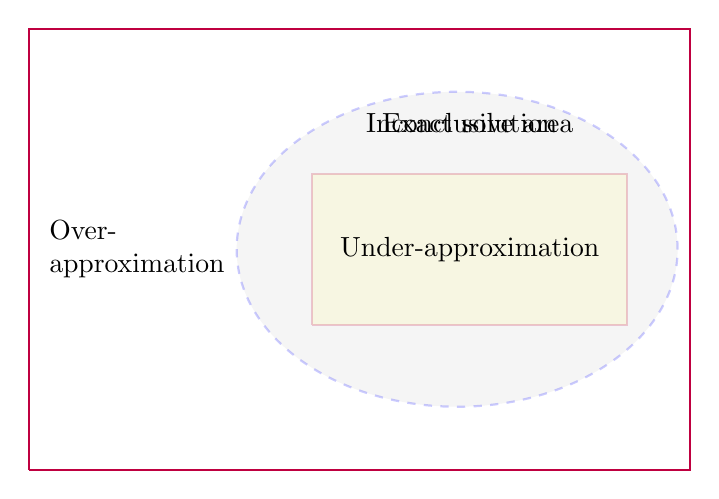
\begin{tikzpicture}[scale=0.8]
  \coordinate (c) at (-0.2,0);
  %\draw<1->[thick,blue,rounded corners=1mm,dashed,fill=gray!40,opacity=0.2] (c) \irregularcircle{3cm}{3mm};
  \draw<1->[thick,blue,rounded corners=1mm,dashed,fill=gray!40,opacity=0.2] (c) ellipse (3.5 and 2.5);
  %\draw[blue] (-1.2,-1.2) -- (1.2,-1.2) -- (1.2,1.2) -- (-1.2,1.2) -- (-1.2,-1.2);
  \draw<3->[thick,purple,fill=yellow!40,opacity=0.2] (-2.5,-1.2) -- (2.5,-1.2) -- (2.5,1.2) -- (-2.5,1.2) -- (-2.5,-1.2);
  \draw<2->[thick,purple] (-7,-3.5) -- (3.5,-3.5) -- (3.5,3.5) -- (-7,3.5) -- (-7,-3.5);
  \node<3-> (under) at (0,0) {Under-approximation};
  \node<2-> [text width=3cm] (over) at (-4.8,0) {Over-\\approximation};
  \node<1> (real) at (0,2) {Exact solution};
  \node<4> (real) at (0,2) {Inconclusive area};
\end{tikzpicture}
%    
%    \vspace{0.5cm}
%    \onslide<5>{$\to$ Apply heuristics on inconclusive area}
%\end{frame}
%
%\begin{frame}{Problematic of Model Inference}
%    \centering
%        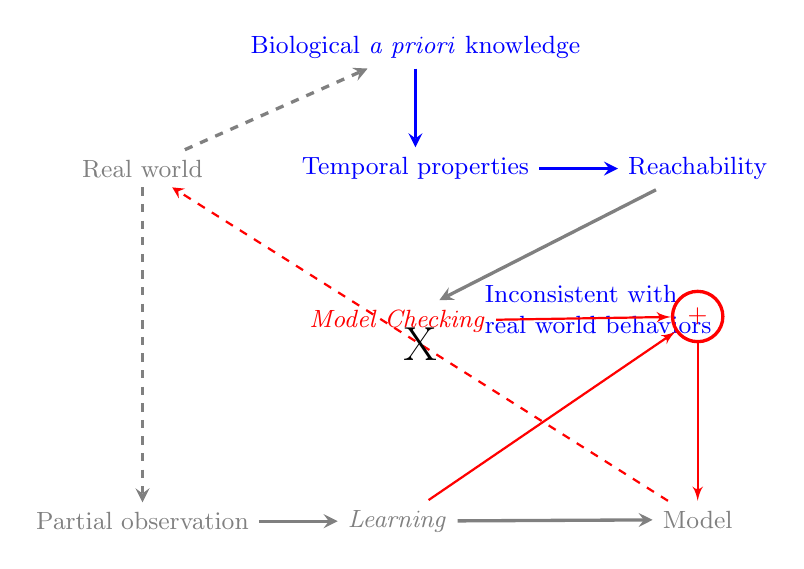
\begin{tikzpicture}[line,>=stealth]
    \small
        \onslide<1->{\node [color=gray] (1) {Real world};}
        \onslide<2->{\node [below = 4cm of 1] (3) {Partial observation};}
        \onslide<2->{\draw [dashed,->] (1) -- (3);}
        \onslide<3->{\node [right = of 3] (4) {\textit{Learning}};}
        \onslide<3->{\draw [->] (3) -- (4);}
        \onslide<7->{\node [color=blue,right = of 1] (2) {Temporal properties};}
        \onslide<8->{\node [color=blue,right = of 2] (5) {Reachability};}
        \onslide<4->{\node [below = 3.95cm of 5] (8) {Model};}
        \onslide<4->{\draw [->] (4) -- (8);}
        \draw<5>[->,thick,dashed,color=red] (8) to node[color=black] {\LARGE X} (1);
        \node<5>[above left = 2cm and -1cm of 8, text width = 3cm, color=blue]{Inconsistent with real world behaviors};
        \onslide<6->{\node [color=blue,above = of 2] (6) {Biological \textit{a priori} knowledge};}
        \onslide<6->{\draw [dashed,->] (1) -- (6);}
        \onslide<8->{\draw [color=blue,->] (2) -- (5);}
        \onslide<7->{\draw [color=blue, ->] (6) -- (2);}
        \onslide<9->{\node [color=red, above = 2cm of 4] (7) {\textit{Model Checking}};}
        \onslide<10->{\node [draw, circle, color = red, above = 2cm of 8] (9) {$+$};}
        \onslide<10->{\draw [thick, color=red] (4) --(9);}
        \onslide<9->{\draw [->] (5) --(7);}
        \onslide<10->{\draw [thick, color=red] (7) --(9);}
        \onslide<11->{\draw [thick, color=red] (9)--(8);}
    \end{tikzpicture}
%\end{frame}
%\begin{frame}{Reachability Problem of Petri Nets}
%    \centering
%    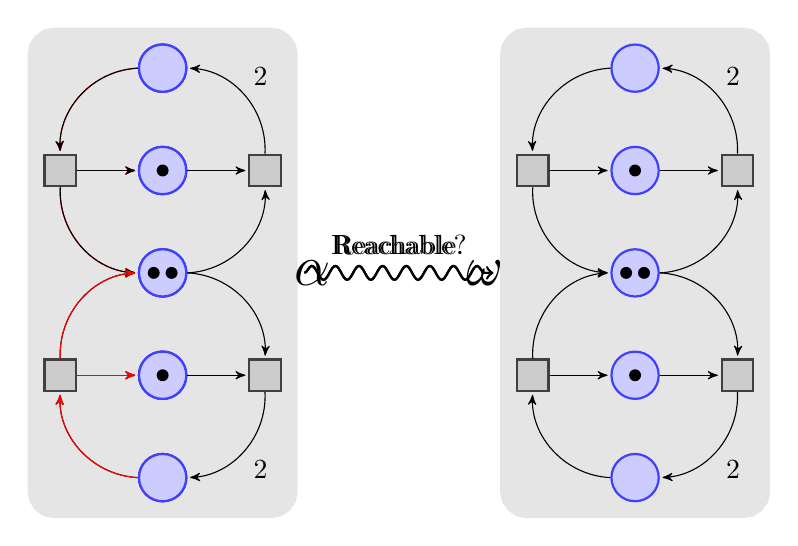
\begin{tikzpicture}[node distance=1.3cm,>=stealth',bend angle=45,auto]

  \tikzstyle{place}=[circle,thick,draw=blue!75,fill=blue!20,minimum size=6mm]
  \tikzstyle{red place}=[place,draw=red!75,fill=red!20]
  \tikzstyle{transition}=[rectangle,thick,draw=black!75,
  			  fill=black!20,minimum size=4mm]

  \tikzstyle{every label}=[red]

  \begin{scope}
    % First net
    \onslide<1,4>{\node [place,tokens=1] (w1)                                    {};
    \node [place] (c1) [below of=w1]                      {};
    \node [place] (s)  [below of=c1] {};
    \node [place] (c2) [below of=s]                       {};
    \node [place,tokens=1] (w2) [below of=c2]                      {};}
    \onslide<2>{\node [place] (w1)                                    {};
    \node [place] (c1) [below of=w1,tokens=1]                      {};
    \node [place] (s)  [below of=c1,tokens=1] {};
    \node [place] (c2) [below of=s]                       {};
    \node [place,tokens=1] (w2) [below of=c2]                      {};}
    \onslide<3>{\node [place] (w1)                                    {};
    \node [place,tokens=1] (c1) [below of=w1]                      {};
    \node [place,tokens=2] (s)  [below of=c1] {};
    \node [place,tokens=1] (c2) [below of=s]                       {};
    \node [place] (w2) [below of=c2]                      {};}

    \node<2> [transition] (e1) [left of=c1] {}
      edge [pre,bend left,color=red]                  (w1)
      edge [post,bend right,color=red]                (s)
      edge [post,color=red]                           (c1);
    \node<1,3,4> [transition] (e1) [left of=c1] {}
      edge [pre,bend left]                  (w1)
      edge [post,bend right]                (s)
      edge [post]                           (c1);

    \node<1,2,4> [transition] (e2) [left of=c2] {}
      edge [pre,bend right]                 (w2)
      edge [post,bend left]                 (s)
      edge [post]                           (c2);
      
    \node<3> [transition] (e2) [left of=c2] {}
      edge [pre,bend right,color=red]                 (w2)
      edge [post,bend left,color=red]                 (s)
      edge [post,color=red]                           (c2);

    \node [transition] (l1) [right of=c1] {}
      edge [pre]                            (c1)
      edge [pre,bend left]                  (s)
      edge [post,bend right] node[swap] {2} (w1);

    \node [transition] (l2) [right of=c2] {}
      edge [pre]                            (c2)
      edge [pre,bend right]                 (s)
      edge [post,bend left]  node {2}       (w2);
  \end{scope}
  
  \begin{scope}[xshift=6cm]
    % First net
    \node [place] (w1')                                    {};
    \node [place,tokens=1] (c1') [below of=w1']                      {};
    \node [place,tokens=2] (s')  [below of=c1'] {};
    \node [place,tokens=1] (c2') [below of=s']                       {};
    \node [place] (w2') [below of=c2']                      {};

    \node [transition] (e1') [left of=c1'] {}
      edge [pre,bend left]                  (w1')
      edge [post,bend right]                (s')
      edge [post]                           (c1');

    \node [transition] (e2') [left of=c2'] {}
      edge [pre,bend right]                 (w2')
      edge [post,bend left]                 (s')
      edge [post]                           (c2');

    \node [transition] (l1') [right of=c1'] {}
      edge [pre]                            (c1')
      edge [pre,bend left]                  (s')
      edge [post,bend right] node[swap] {2} (w1');

    \node [transition] (l2') [right of=c2'] {}
      edge [pre]                            (c2')
      edge [pre,bend right]                 (s')
      edge [post,bend left]  node {2}       (w2');
  \end{scope}

  \onslide<1,2>{\draw [-to,thick,decorate, decoration=snake, segment length=3mm]
    ([xshift=5mm]s -| l1) -- ([xshift=-5mm]s' -| e1')
    node [above=1mm,midway,text width=3cm,text centered]
      {Reachable?};}
  \onslide<3>{\draw [-to,thick,decorate, decoration=snake, segment length=3mm]
    ([xshift=5mm]s -| l1) -- ([xshift=-5mm]s' -| e1')
    node [above=1mm,midway,text width=3cm,text centered]
      {Reachable.};}
  \onslide<4>{\node (alpha) at ([xshift=6mm]s -| l1) {\huge$\alpha$};
  \node (alpha) at ([xshift=-6mm]s' -| e1') {\huge$\omega$};}
  \begin{pgfonlayer}{bg}
    \filldraw [line width=4mm,rounded corners,black!10]
      (w1.north  -| l1.east)  rectangle (w2.south  -| e1.west)
      (w1'.north -| l1'.east) rectangle (w2'.south -| e1'.west);
      
  \end{pgfonlayer}
\end{tikzpicture}    
%\end{frame}

\begin{frame}{Reachability Problem of State Space}
    \centering
    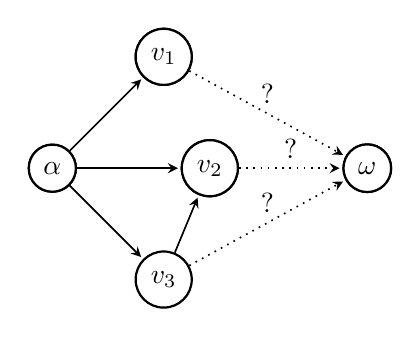
\begin{tikzpicture}[
        > = stealth, % arrow head style
        shorten > = 1pt, % don't touch arrow head to node
        auto,
        node distance = 2cm, % distance between nodes
        semithick % line style
    ]

    \tikzstyle{every state}=[
        draw = black,
        thick,
        fill = white,
        minimum size = 4mm
    ]

    \node<1>[state,fill=blue!30] (s) {$\alpha$};
    \node<2->[state] (s) {$\alpha$};
    \node<3>[state] (v1) [above right of=s,fill=blue!30] {$v_1$};
    \node<1,2,4->[state] (v1) [above right of=s] {$v_1$};
    \node<2>[state] (v2) [right of=s,fill=blue!30] {$v_2$};
    \node<1,3->[state] (v2) [right of=s] {$v_2$};
    \node[state] (v3) [below right of=s] {$v_3$};
    \node<4->[state] (t) [right of=v2,fill=blue!30] {$\omega$};
    \node<1-3>[state] (t) [right of=v2] {$\omega$};

    \draw[->] (s) -- (v1);
    \draw[->] (s) -- (v2);
    \draw[->] (s) -- (v3);
    \draw[->] (v3) -- (v2);
    \draw[->,dotted] (v1) -- node [above,midway] {?} (t);
    \draw[->,dotted] (v2) -- node [above,midway] {?} (t);
    \draw[->,dotted] (v3) -- node [above,midway] {?} (t);
\end{tikzpicture}
    $\alpha \to\cdots \to\omega?$
\end{frame}
\begin{frame}
\begin{itemize}
    \item Hybrid analyzer is more performing in reachability analysis
\end{itemize}
What are the capabilities and limits of your experiment? How often do the things that your experiment does come up in the real world? What's involved in extending it? If it's easy to extend, why haven't you? If your example is a piece of a larger system, how realistic are your assumptions about input and output?

\end{frame}




\end{document}
